\documentclass[main.tex]{subfiles}

% Document
\begin{document}

\chapter{Simulating a mass on a spring}

\section{Introduction}

In Part 1, we put together a general function for timestepping a differential equation, and several different integrator methods to use along with it.
In this section, we'll start running them on a first test problem to get used to running simulations and assessing their accuracy.

\section{Setting up the equations}

\begin{figure}
\centering
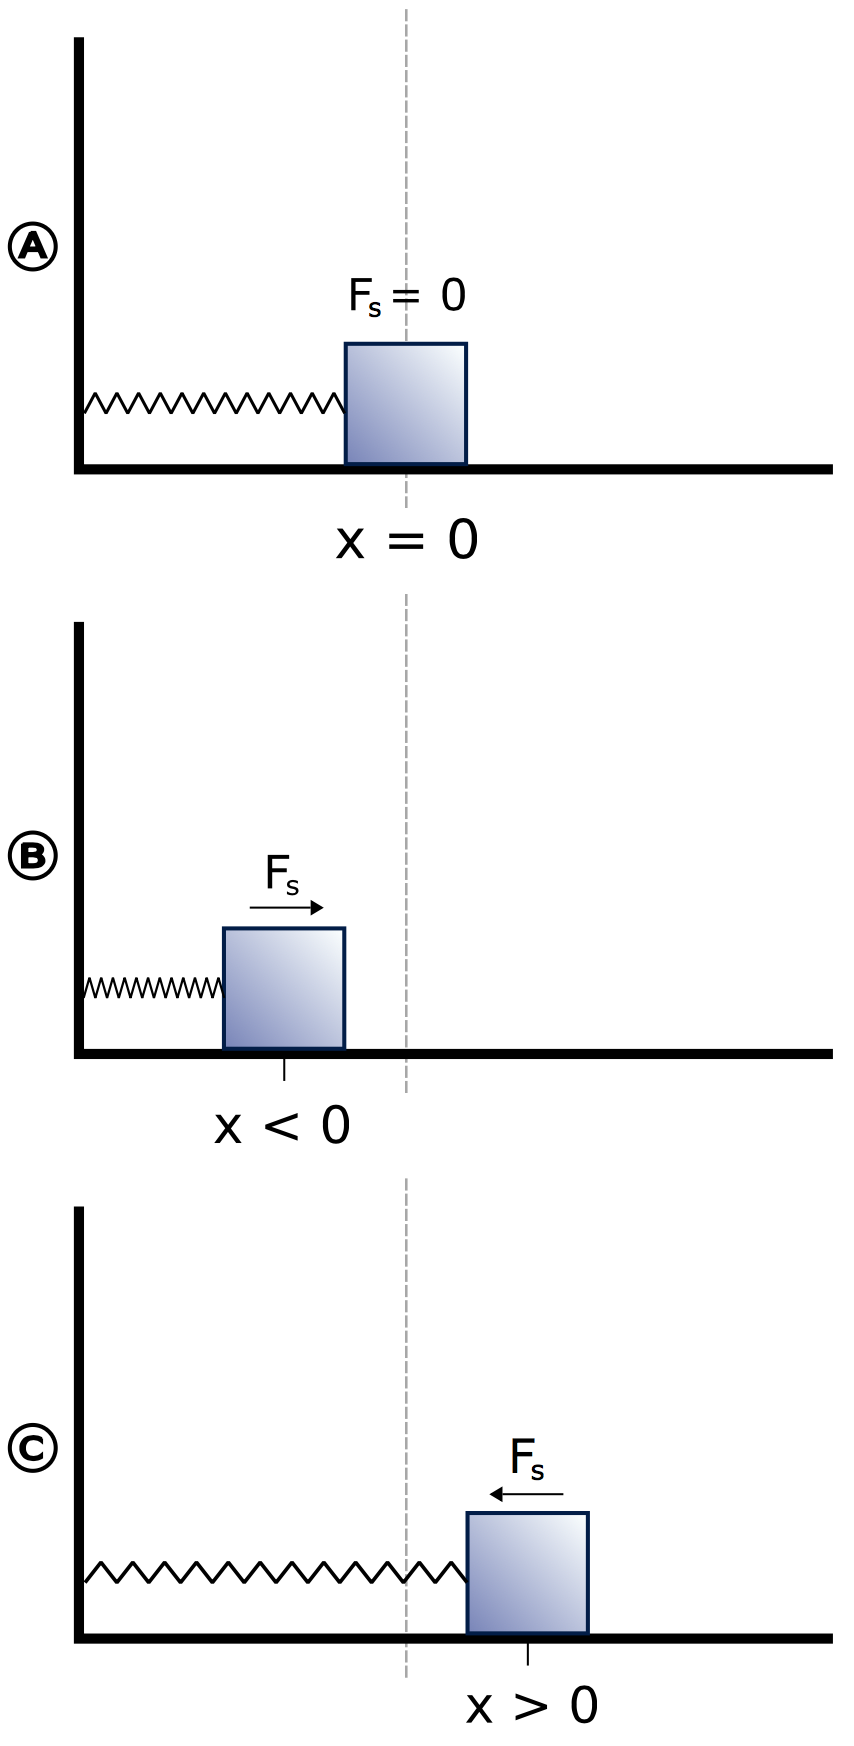
\includegraphics[width=0.4\textwidth]{images/mass}
\caption{Spring-mass system in equilibrium (A), compressed (B), and stretched (C) states. (Wikipedia)}
\end{figure}

The first system we'll simulate is the one-dimensional motion of a mass attached to a horizontal spring (see image).
Hooke's law for a spring tells us that the force exerted by the spring is proportional to the distance that it is stretched or compressed.
If $x(t)$ is the position of the mass at time $t$, and the equilibrium position is at $x=0$, then the force $F_s$ of the spring on the mass is written as

\begin{equation}
    F_s = - k x
\end{equation}

Newton's laws tell us that when a force is applied to an object, it accelerates with an acceleration equation to the force divided by the object's mass, so the acceleration of the mass should be

\begin{equation}
    a = \frac{F_s}{m}
\end{equation}

As we discussed in section 1.3.2, since the acceleration is the second derivative of the position in time, we'll need to construct a system of two equations to numerically solve this problem.

Task 7: Write out the system of equations for the motion of a mass on a spring.
You'll need to specify the variables that make up the vector of unknowns, $U$, along with the functions in $F$ that give the time-derivatives of the unknowns.

\section{Running a simulation}

Now that we have the system of equations written down, we need to code-up the function $F$ so we can pass it to our timestepper.

Task 8: Write a Python function, matching the interface specified in Task 3, that returns the time-derivative system for the motion of a mass on a spring.

Hints:
\begin{itemize}
\item The function should accept as its arguments an array $U_n$ of the unknown variables, and the time $t_n$.
\item It might be helpful to unpack the variables from the input array before constructing the output array.
Unpacking can be done with the syntax
\begin{python}
 x, v = U
\end{python}
which is just a compact way of writing
\begin{python}
 x = U[0]
 v = U[1]
\end{python}
\item To keep things simple, let's start by setting $k=1$ and $m=1$.
\end{itemize}

Next we need to specify our initial conditions in a vector $A$.
Let's start out by setting the initial position to $x_0=1$, and the initial velocity to $v_0=0$.
Now let's run our first simulation!

Task 9: 
Simulate the mass on the spring to a final time $T=10$ using the Euler integrator.
What step-size $h$ do you think we should use?
Pick something and try it!
After specifying all the necessary variables, you can run the simulation and plot the results in a notebook using the following code (which might need to be tweaked to match your variable names!):

\begin{python}
 t, U = timestep(A, F_spring, euler, T, h)
 plt.figure(figsize=(10,6))
 plt.plot(t, U[:,0], '.-')
 plt.xlabel('t')
 plt.ylabel('x')
\end{python}

The first line here runs the simulation.
The next lines create a figure, plot the first unknown (position) against time, and put some labels on the plot.

Alright!
That's our first simulation!
Depending on the timestep you picked, the numerical solution might be really good, or pretty bad!
Let's see what happens when we twist the knobs.

Task 10:
Experiment with all the different parameters.
Some things to look at include:
\begin{itemize}
\item What happens when you change the step-size?  What step-size seems to be good enough?
\item What happens if you change the initial position and velocity?
\item What happens if you change the spring constant or the mass?
\item What happens if you use a different integrator?
\end{itemize}

\section{Computing the error}

Now that we have a feel for how the numerical solutions behave as we change the numerical settings (step-size and integrator), we'll perform a more quantitative analysis of the accuracy of our simulations.

The problem we've chosen is an example of harmonic motion, meaning the solution can be written out analytically in terms of sine and cosine functions.
In particular, the solution should repeat with a period given by

\begin{equation}
    P = \frac{2 m}{k}
\end{equation}

To assess the accuracy of our algorithms, we can therefore run a simulation for a full period, and compare the final position of the mass with the initial position we used to start the simulation.

Task 11:
Write a function that returns the error in the position of the mass after one period.
The function should accept the step-size and the integrator as arguments.
Try the function with a few values of the time-step and the different integrators.
Do the results make sense?
If we want the simulation to end at exactly one period, is there any restriction on how we should choose the step-size $h$?

\section{Comparing integrators}

We've seen that for a given step-size, the different integrators will produced solutions with different errors.
If we want to adjust the step-size to produce a solution with an error less than some set tolerance (say, we want to know the proper position to within $\Delta x = 10^{-6}$, we need to know the rate at which the error decreases as we make the step-size smaller.
This rate is called the rate of convergence of the integrator.

Task 12:
Calculate the error for each integrator over a range of step-sizes, and plot the results.
Which method has the fastest rate of convergence?
Which has the slowest?
Is this what you expected?
Why or why not?

Hints:
\begin{itemize}
\item A good set of timesteps to use might be something like
\begin{python}
 H = 2*np.pi / 2**np.arange(4,12)
\end{python}
which is an array of step-sizes that divide the period by different powers of two.
\item The best way to plot the display the data is probably to plot the logarithm of the absolute value of the error against the logarithm of the time-step.
Try the \pyth{plt.loglog} function.
\end{itemize}

What do you think will happen if we keep decreasing the step-size forever?
The answer turns out to depend on the way computers represent real numbers, which is a system called floating-point arithmetic.
This system can represent numbers from roughly $-10^{308}$ to $+10^{308}$, but with only about 16 digits of precision.
So if you're adding some number to another one that's much larger, the computer's representation may not be precise enough to track the difference.

Task 13:
Rerun task 12, but with lower and lower minimum step-sizes.  
Can you find the precision floor for one of the integrators?  
At what amplitude, roughly, does it occur?  
Does this level make sense, given the information above on the floating-point system?

\section{Conclusion}

With some successful simulations under our belt, we're ready to push on to more complicated problems.  
In many cases, we won't know what the solution should look like, so we won't be able to simply calculate the error in our numerical simulations, as we did for the mass-spring system here.  
Instead, we've have to use some of our experience from this test problem to pick the write integrator and parameters to produce reliable solutions, when we don't know what the answer should be!

\end{document}
